\documentclass{boi2014-pl}

\usepackage{enumitem}
\usepackage{todonotes}
\usepackage{wrapfig}
\usepackage{mathtools}
\usepackage{tikz}

\renewcommand{\DayNum}{1}
\renewcommand{\TaskCode}{coprobber}
\renewcommand{\TaskName}{Policjant i złodziej}

\renewcommand{\labelitemii}{$\circ$}
\newcommand{\param}[1]{{\tt #1}}
\renewcommand{\method}[1]{{\tt #1}}
\newcommand{\constant}[1]{{\tt #1}}

\begin{document}
    Przestępczość w Bajtogrodzie jest na porządku dziennym.
    Szczególnie często mają miejsce kradzieże.
    Jedną z przyczyn tego stanu rzeczy może być fakt, iż w pogoń za złodziejem
    rusza zazwyczaj tylko jeden policjant znajdujący się akurat w terenie.
    Pościg w starościeckim stylu odbywa się wąskimi uliczkami łączącymi
    \emph{skrzyżowania} Bajtogrodu, więc dzięki dobrej znajomości miasta złodziejowi
    nierzadko udaje się umknąć policjantowi.

    Komenda Stołeczna Policji w Bajtogrodzie (KSPB) organizuje zgrupowanie poświęcone
    zmniejszeniu skali przestępczości w mieście.
    Jednym z pomysłów jest wprowadzenie automatycznego systemu planowania tras pościgu.
    Pierwszym krokiem było zdobycie przez KSPB precyzyjnego planu miasta.
    Teraz poproszono Cię, abyś przygotował program, który korzystając z tych danych,
    umożliwi efektywne planowanie pościgu.

    Pościg policjanta za złodziejem modelujemy następująco:
    \begin{enumerate}
        \item Policjant wybiera skrzyżowanie, na którym rozpoczyna swój patrol.
        \item Następnie złodziej wybiera skrzyżowanie, przy którym dokona włamania
            (zna on skrzyżowanie, na którym znajduje się policjant).
            Od tego momentu zakładamy, że policjant i złodziej znają wzajemnie
            swoje położenia.
        \item W pojedynczym ruchu policjant przemieszcza się na sąsiednie skrzyżowanie
            (tzn.\ skrzyżowanie połączone bezpośrednio uliczką ze skrzyżowaniem,
            na którym jest obecnie) lub decyduje się czekać (tzn.\ nie przemieszcza się).
        \item W pojedynczym ruchu złodziej przemieszcza się na sąsiednie skrzyżowanie.
            Zauważ, że w przeciwieństwie do policjanta, złodziej nigdy nie czeka
            w swoim ruchu.
            Na złodzieju czapka gore.
        \item Policjant i złodziej wykonują ruchy na przemian (począwszy od policjanta),
            aż do momentu, gdy:
        \begin{enumerate}
            \item wcześniejsza sytuacja powtórzy się (przez sytuację rozumiemy pozycje
                obu postaci oraz to, do którego gracza należy najbliższy ruch).
                Wówczas złodziej może unikać spotkania z policjantem w nieskończoność,
                więc przyjmujemy, że złodziej ucieka; albo
            \item policjant i złodziej spotykają się na tym samym skrzyżowaniu
                po ruchu któregoś z nich.
                Wówczas policjant łapie złodzieja.
        \end{enumerate}
    \end{enumerate}

    \Task
    Napisz program, który mając dany plan miasta, stwierdzi, czy policjant może
    złapać złodzieja, a jeśli tak, przeprowadzi pościg w imieniu policjanta.

    Twój program powinien założyć, że złodziej porusza się w sposób optymalny.

    \Implementation
    Powinieneś zaimplementować dwie funkcje:
    \begin{itemize}
        \item \method{start(N, A)} o następujących parametrach:
            \begin{itemize}
                \item $N$ --- liczba skrzyżowań (skrzyżowania są ponumerowane od $0$ do $N-1$)
                \item $A$ --- dwuwymiarowa tablica opisująca uliczki;
                    dla $0 \le i, j \le N-1$,
                    $$
                        A[i, j] \text{ jest równe }
                        \begin{dcases*}
                            \texttt{false} & jeśli $i$ oraz $j$ nie są połączone uliczką
                                \\
                            \texttt{true} & jeśli $i$ oraz $j$ są połączone uliczką
                        \end{dcases*}
                    $$
                    Wszystkie uliczki są dwukierunkowe (tzn.\ $A[i, j] = A[j, i]$
                    dla wszystkich $i$ oraz $j$) i każda uliczka łączy dwa różne skrzyżowania
                    (tzn.\ $A[i, i]$ będzie równe \texttt{false} dla wszystkich $i$).
                    Możesz ponadto założyć, że za pomocą systemu uliczek można przedostać
                    się z dowolnego skrzyżowania na dowolne inne skrzyżowanie.
            \end{itemize}

        Jeśli w tak opisanym mieście policjant może złapać złodzieja,
        wynikiem funkcji \method{start} powinien być numer skrzyżowania,
        na którym policjant powinien rozpocząć swój patrol.
        W przeciwnym razie wynikiem funkcji powinno być $-1$.

        \item \method{nextMove(R)} przyjmującą jako parametr liczbę
            $R$ oznaczającą numer skrzyżowania, przy którym znajduje się złodziej
            i zwracającą numer skrzyżowania, przy którym policjant znajdzie się
            po wykonaniu swojego ruchu.
    \end{itemize}

    Funkcja \method{start} zostanie wywołana dokładnie raz,
    przed wszystkimi wywołaniami funkcji \method{nextMove}.
    Jeśli wynikiem funkcji \method{start} będzie $-1$,
    funkcja \method{nextMove} nie będzie wywoływana.
    W przeciwnym razie, funkcja \method{nextMove} będzie wywoływana w kółko
    aż do końca pościgu.
    Program zakończy się, gdy nastąpi jeden z poniższych warunków:
    \begin{itemize}
        \item funkcja \method{nextMove} zwróci niepoprawny ruch;
        \item wcześniejsza sytuacja powtórzy się;
        \item złodziej zostanie złapany.
    \end{itemize}

    \Example
    \begin{wrapfigure}[4]{r}{2cm}
        \vspace{-0.5cm}
        \centering
        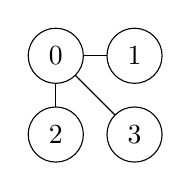
\begin{tikzpicture}
        \draw (0,1) -- (0,0);
        \draw (0,1) -- (1,0);
        \draw (0,1) -- (1,1);
        \foreach \x in {0,1} \foreach \y in {0,1}
            \draw (\x,\y) node[circle,draw,fill=white,inner sep=0,minimum size=0.7cm] {\pgfmathparse{int(2-2*\y+\x)}\pgfmathresult};
        \end{tikzpicture}
    \end{wrapfigure}
    Przyjrzyjmy się przykładowi opisanemu przez obrazek po prawej stronie.
    W tym przykładzie każde skrzyżowanie jest dobrą pozycją początkową dla policjanta.
    Jeśli policjant rozpocznie przy skrzyżowaniu numer 0, w swoim pierwszym ruchu
    może postanowić poczekać -- wówczas złodziej sam na niego wpadnie.
    Jeśli zaś policjant rozpocznie przy jakimkolwiek innym skrzyżowaniu, może poczekać,
    aż złodziej znajdzie się przy skrzyżowaniu numer 0, i wówczas przejść na to skrzyżowanie.
   
    Oto jedno z możliwych wykonań programu dla tego przykładu:

    \begin{tabular}{|l|c|}
        \hline
            {\bf Wywołanie funkcji} & {\bf Wynik} \\
        \hline
            \method{start(4, [[0, 1, 1, 1], [1, 0, 0, 0], [1, 0, 0, 0], [1, 0, 0, 0]])} &
            \constant{3} \\
        \hline
            \method{nextMove(1)} & \constant{3} \\
        \hline
            \method{nextMove(0)} & \constant{0} \\
        \hline
    \end{tabular}

    \Scoring
    Aby uzyskać pełną punktację, Twoje rozwiązanie musi:
    In order to score full points, your solution must:
    \begin{enumerate}
      \item poprawnie stwierdzić, czy policjant może złapać złodzieja;
      \item skutecznie złapać złodzieja, wykonując ruchy w imieniu policjanta.
    \end{enumerate}
   
    Jednakże w podzadaniach 3 i 4, rozwiązania, które spełniają tylko pierwsze
    w powyższych wymagań, uzyskają 30\% punktów za odpowiednie podzadanie.

    \begin{description}
        \item[Podzadanie 1 (15 punktów):] $2 \le N \le 500$. Między każdą parą skrzyżowań jest dokładnie jedna ścieżka.
        \item[Podzadanie 2 (15 punktów):] $2 \le N \le 500$. Sieć skrzyżowań i uliczek tworzy kratkę.
        Kratka składa się z co najmniej dwóch wierszy i kolumn, a numeracja skrzyżowań
        odpowiada schematowi przedstawionemu na rysunku poniżej.
        \begin{figure}[h!]
           \centering
           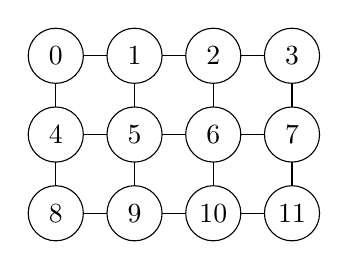
\begin{tikzpicture}
            \draw (0,0) grid (3,2);
            \foreach \x in {0,1,2,3} \foreach \y in {0,1,2}
                \draw (\x,\y) node[circle,draw,fill=white,inner sep=0,minimum size=0.7cm] {\pgfmathparse{int(8-4*\y+\x)}\pgfmathresult};
           \end{tikzpicture}
        \end{figure}
        \item[Podzadanie 3 (30 punktów):] $2 \le N \le 100$.
        \item[Podzadanie 4 (40 punktów):] $2 \le N \le 500$.
    \end{description}

    \Constraints
    
    \begin{description}
        \item[Limit czasu:] 1 s.
        \item[Dostępna pamięć:] 256 MB.
    \end{description}

    \todo{Need to add info about graders.}
\end{document}
